
\section{Methodology}
\label{sec:methodology}
\todo{This section is should be more of a high level discussion about methods used, why we chose them and the system/game}

\ravjot{Feel free to use this to make comments in the paper you want me to look at.}

\glen{I will use this}

	In this section we outline our solution to our distributed state synchronization design. We discus what protocols are used, how the clients and servers communicate and the example game constructed for this system.
	
\subsection{The Clients}

	The client locally simulates its own version of the game. To support this the client needs to keep a list of the agents controlled by other clients in the game and the most recent location of each agent. This information will be stored in a \emph{hashmap}. After every frame is rendered in the game the client will broadcast a position update to all servers.
	
\subsection{The Servers}

	The server simulates its own version of the game. The server is not used just to reduce message passing but also to act as an authority over clients, to prevent malicious clients from propagating invalid information.
	
	In the simulation loop for the server a number of actions occur
	\begin{enumerate}[topsep=2pt,itemsep=-1ex,partopsep=1ex,parsep=1ex]
		\item the server accepts event messages and puts them in a queue for processing
		\item The server accepts position updates from clients
		\item The server verifies these updates to be valid
		\item The server's local copy of agent locations is updated
		\item The server processes any events in its event queue
		\item If events are valid, update server's game state and broadcast the result
	\end{enumerate}
	
	This way the server keeps the true state of the game and informs the clients of valid updates to the server's state. To perform these operations the server needs to have state for the currently active clients and its own version of the game state.

\subsection{The Activity Server}
	The purpose of Activity Server is to support the architecture of the System which includes allowing a new node to join th system and publishing the list of nodes which are currently online. The Activity Server doesn't do any kind og game simulation niether involves in game semantic actions.

\subsection{The KV-Service}
	The KV-Service is a key-value service which used for all communication among the nodes and the activity server that is required to maintain the system. The servers periodically update their entry in the KV-Service. The activity server polls with twice the period rest of the servers are polling. The activity server read the entries of all the nodes and publish a list of nodes including all those nodes who have recently updated their entry. 

\subsection{ARM Game}

	We will simulate a very basic game to use as our state to synchronize. 
	The game has two possible actions \move{\agent}{\position} and \fire{\agent_{i}}{\agent_{j}}. These actions can be executed at any point in the game but the server must validate the actions. 
	
	In order to simulate the game, information is needed on the other agents in the game. The only data stored for each agent is the agent's current location. The information needed for the game will be provided from the server or client the game is being simulated on. Computer animations and therefore game simulations use simulation time, similar to a vector clock, for synchronizing events.
	
\subsubsection{Protocol and Messaging}

	The clients send updates/events to every server. For \fire{\agent_{i}}{\agent_{j}} events the server that is paired with the client with $\agent_{j}$ will determine the outcome. If the \fire{\agent_{i}}{\agent_{j}} event is successful according to the authoritative server a \destroy{\agent_{j}} event is broadcast to every server. All communication is asynchronous without acknowledgements, except for the \destroy{\agent_{j}} event.


\subsection{Distributed Servers}
\label{subsec:distributed-servers}

	We construct a distributed server model (see Figure~\ref{figure:server-models}(b)) to enable better failure handling in our system. Each client is paired with a server which is running on the same machine. The paired server validates the actions performed by client and process it further if the action is found valid. The authoritative server for a particular client depends on the event/action being processed. 
	
	\begin{figure}[ht]
	\centering
	\begin{tabular}{c c}
		Client-Server & Distributed Server \\
		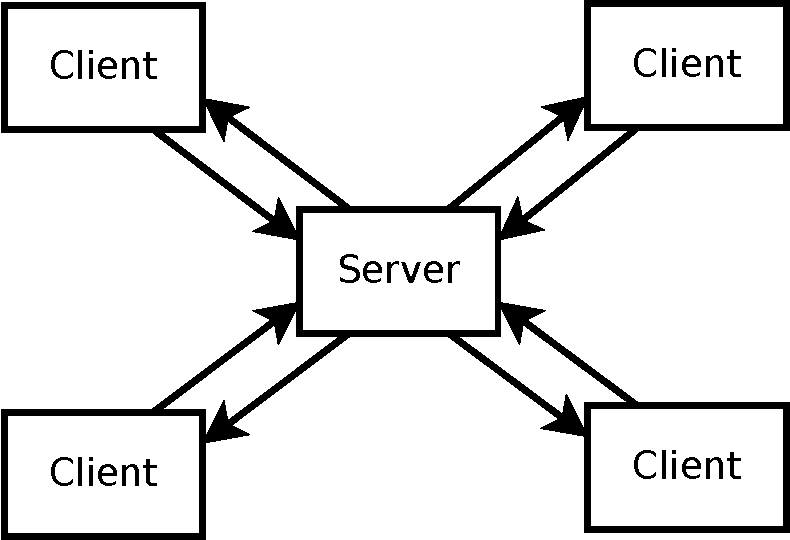
\includegraphics[width=0.44\linewidth]{../images/client-server-model-crop.pdf} &
		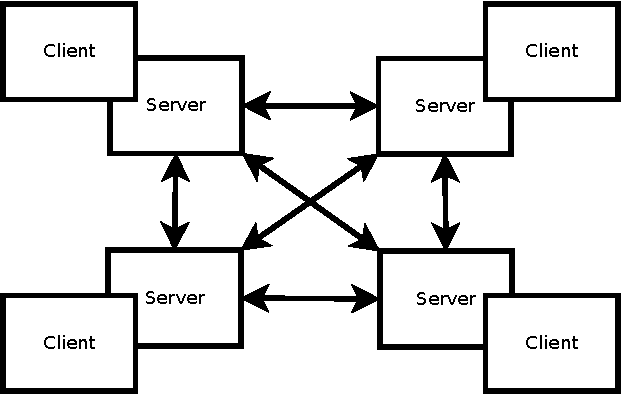
\includegraphics[width=0.48\linewidth]{../images/client-distributed-server-model-crop.pdf} \\
		(a) & (b)
	\end{tabular}

	\caption{\label{figure:server-models} The first model (a) is an example \clientServer model. In this model all of the clients send updates to the server and the server send updates out to the clients. In the second model (b) the server is distributed and clients communicate with many servers.}
	\end{figure}
	
